\documentclass[10pt,twocolumn]{article}

\usepackage[a4paper,margin=1.8cm]{geometry}
\usepackage{graphicx}
\usepackage{amsmath}
\usepackage{booktabs}
\usepackage{hyperref}
\usepackage{float}

\title{COVID-19 Infection Segmentation Using Deep Learning}
\author{Minh Pham Nhat}

\begin{document}

\maketitle

\begin{abstract}
This report presents a deep learning approach for COVID-19 infection segmentation from medical images. 
The objective is to detect infection regions using a convolutional neural network trained on annotated 
medical images. The dataset characteristics, model implementation, experimental results, and comparison 
with existing state-of-the-art approaches are discussed. Hyperparameter experiments are also conducted 
to evaluate their impact on model performance.
\end{abstract}

\section{Introduction}

The COVID-19 pandemic has motivated the development of automated tools to assist medical diagnosis. 
Deep learning methods, particularly convolutional neural networks (CNNs), have shown strong performance 
in medical image segmentation tasks. In this project, we implement a deep learning model to segment 
infection regions from medical images using a supervised learning framework.

The objectives of this study include:

\begin{itemize}
\item Describing the dataset used for training and evaluation
\item Implementing a deep learning segmentation model
\item Comparing results with existing methods
\item Evaluating the effect of different hyperparameters
\end{itemize}

\section{Dataset Description}

The dataset used in this project is the \textbf{COVID-QU-Ex} dataset. 
It is organized into three main subsets:

\begin{itemize}
\item \textbf{Train}
\item \textbf{Validation (Val)}
\item \textbf{Test}
\end{itemize}

The directory structure of the dataset is shown below:

Each subset contains chest X-ray images categorized into three clinical classes:

\begin{itemize}
\item \textbf{COVID-19} – X-ray images of patients infected with COVID-19
\item \textbf{Non-COVID} – X-ray images of patients with lung diseases other than COVID-19
\item \textbf{Normal} – X-ray images of healthy lungs
\end{itemize}

This folder-based structure allows the dataset to be easily loaded using common 
deep learning libraries such as \texttt{PyTorch} or \texttt{TensorFlow} through 
standard image dataset loaders.

The images are medical chest X-ray scans that represent different lung conditions. 
During preprocessing, the images are resized and normalized before being used as 
inputs to the deep learning model.

The dataset is divided into training, validation, and test sets to allow proper 
model training, hyperparameter tuning, and unbiased performance evaluation.


\section{Model Implementation}

The segmentation model implemented in this project is an \textbf{Attention U-Net} architecture 
developed using the PyTorch deep learning framework. The network follows an encoder–decoder 
structure with skip connections, enhanced with residual convolution blocks and attention gates 
to improve feature propagation and focus on relevant regions of the lungs.

\subsection{Basic Convolution Blocks}

Several modular building blocks are defined to construct the network.

\textbf{ConvBNReLU Block}

This block consists of a convolution layer followed by batch normalization and a ReLU activation:

\begin{itemize}
\item Convolution ($3\times3$ kernel)
\item Batch Normalization
\item ReLU activation
\end{itemize}

This block helps stabilize training and improves gradient flow.

\textbf{Double Convolution Block}

The \texttt{DoubleConv} module applies two consecutive convolution layers:

\begin{equation}
Conv \rightarrow BN \rightarrow ReLU \rightarrow Conv \rightarrow BN \rightarrow ReLU
\end{equation}

This block extracts richer spatial features from the input images.

\textbf{Residual Double Convolution}

A residual version of the double convolution block is implemented to improve training stability:

\begin{equation}
Output = F(x) + x
\end{equation}

where $F(x)$ represents the stacked convolution operations.  
Residual connections help prevent vanishing gradients and allow deeper feature learning.

\subsection{Upsampling Module}

The decoder uses an \textbf{UpConv} module to increase spatial resolution.  
This module performs:

\begin{itemize}
\item Bilinear upsampling
\item Convolution for channel adjustment
\end{itemize}

The upsampled feature maps are then concatenated with encoder features through skip connections.

\subsection{Attention Gates}

Attention mechanisms are introduced through the \texttt{AttentionGate} module.  
The attention gate receives two inputs:

\begin{itemize}
\item $g$ : gating signal from the decoder
\item $x$ : feature map from the encoder
\end{itemize}

The gate learns attention coefficients that suppress irrelevant background features and highlight 
important regions in the lungs before concatenation with the decoder features.

This mechanism allows the model to focus more effectively on infection regions.

\subsection{Attention U-Net Architecture}

The full model is implemented in the \texttt{AttentionUNet} class.

The architecture contains:

\begin{itemize}
\item Encoder path for feature extraction
\item Bottleneck layer
\item Decoder path for segmentation reconstruction
\item Attention gates applied to skip connections
\end{itemize}

The encoder progressively reduces spatial resolution while increasing the number of feature channels.  
The decoder restores the spatial resolution using upsampling layers and skip connections.

The model is initialized as:

\begin{verbatim}
AttentionUNet(
    in_channels = 1,
    num_classes = 3
)
\end{verbatim}

The three output classes correspond to:

\begin{itemize}
\item COVID-19 infected regions
\item Non-COVID lung abnormalities
\item Normal lung tissue
\end{itemize}

\subsection{Loss Function}

To improve segmentation performance, a custom Dice-based loss is implemented:

\begin{equation}
Dice = \frac{2|P \cap G|}{|P| + |G|}
\end{equation}

where:

\begin{itemize}
\item $P$ is the predicted mask
\item $G$ is the ground truth mask
\end{itemize}

The Dice loss encourages better overlap between predicted and ground-truth segmentation regions.

In the experiments, the Dice loss is combined with cross-entropy loss to balance pixel-wise 
classification and region-level overlap.


\section{Training Procedure}

The model is double-trained with both CrossEntropy and DiceCE loss function using the following configuration:

\begin{itemize}
\item Optimizer: Adam
\item Learning rate: 0.001
\item Batch size: 32
\item Number of epochs: 10
\end{itemize}

Training is performed using GPU acceleration when available.

The evaluation metrics include:

\begin{itemize}
\item Mean Abosulute Error (MAE)
\item Intersection over Union (IoU)
\item Accuracy
\end{itemize}

\section{Results}

Figure 1 and 2 shows examples of predicted infection masks compared with the ground truth.

\begin{figure}[H]
\centering
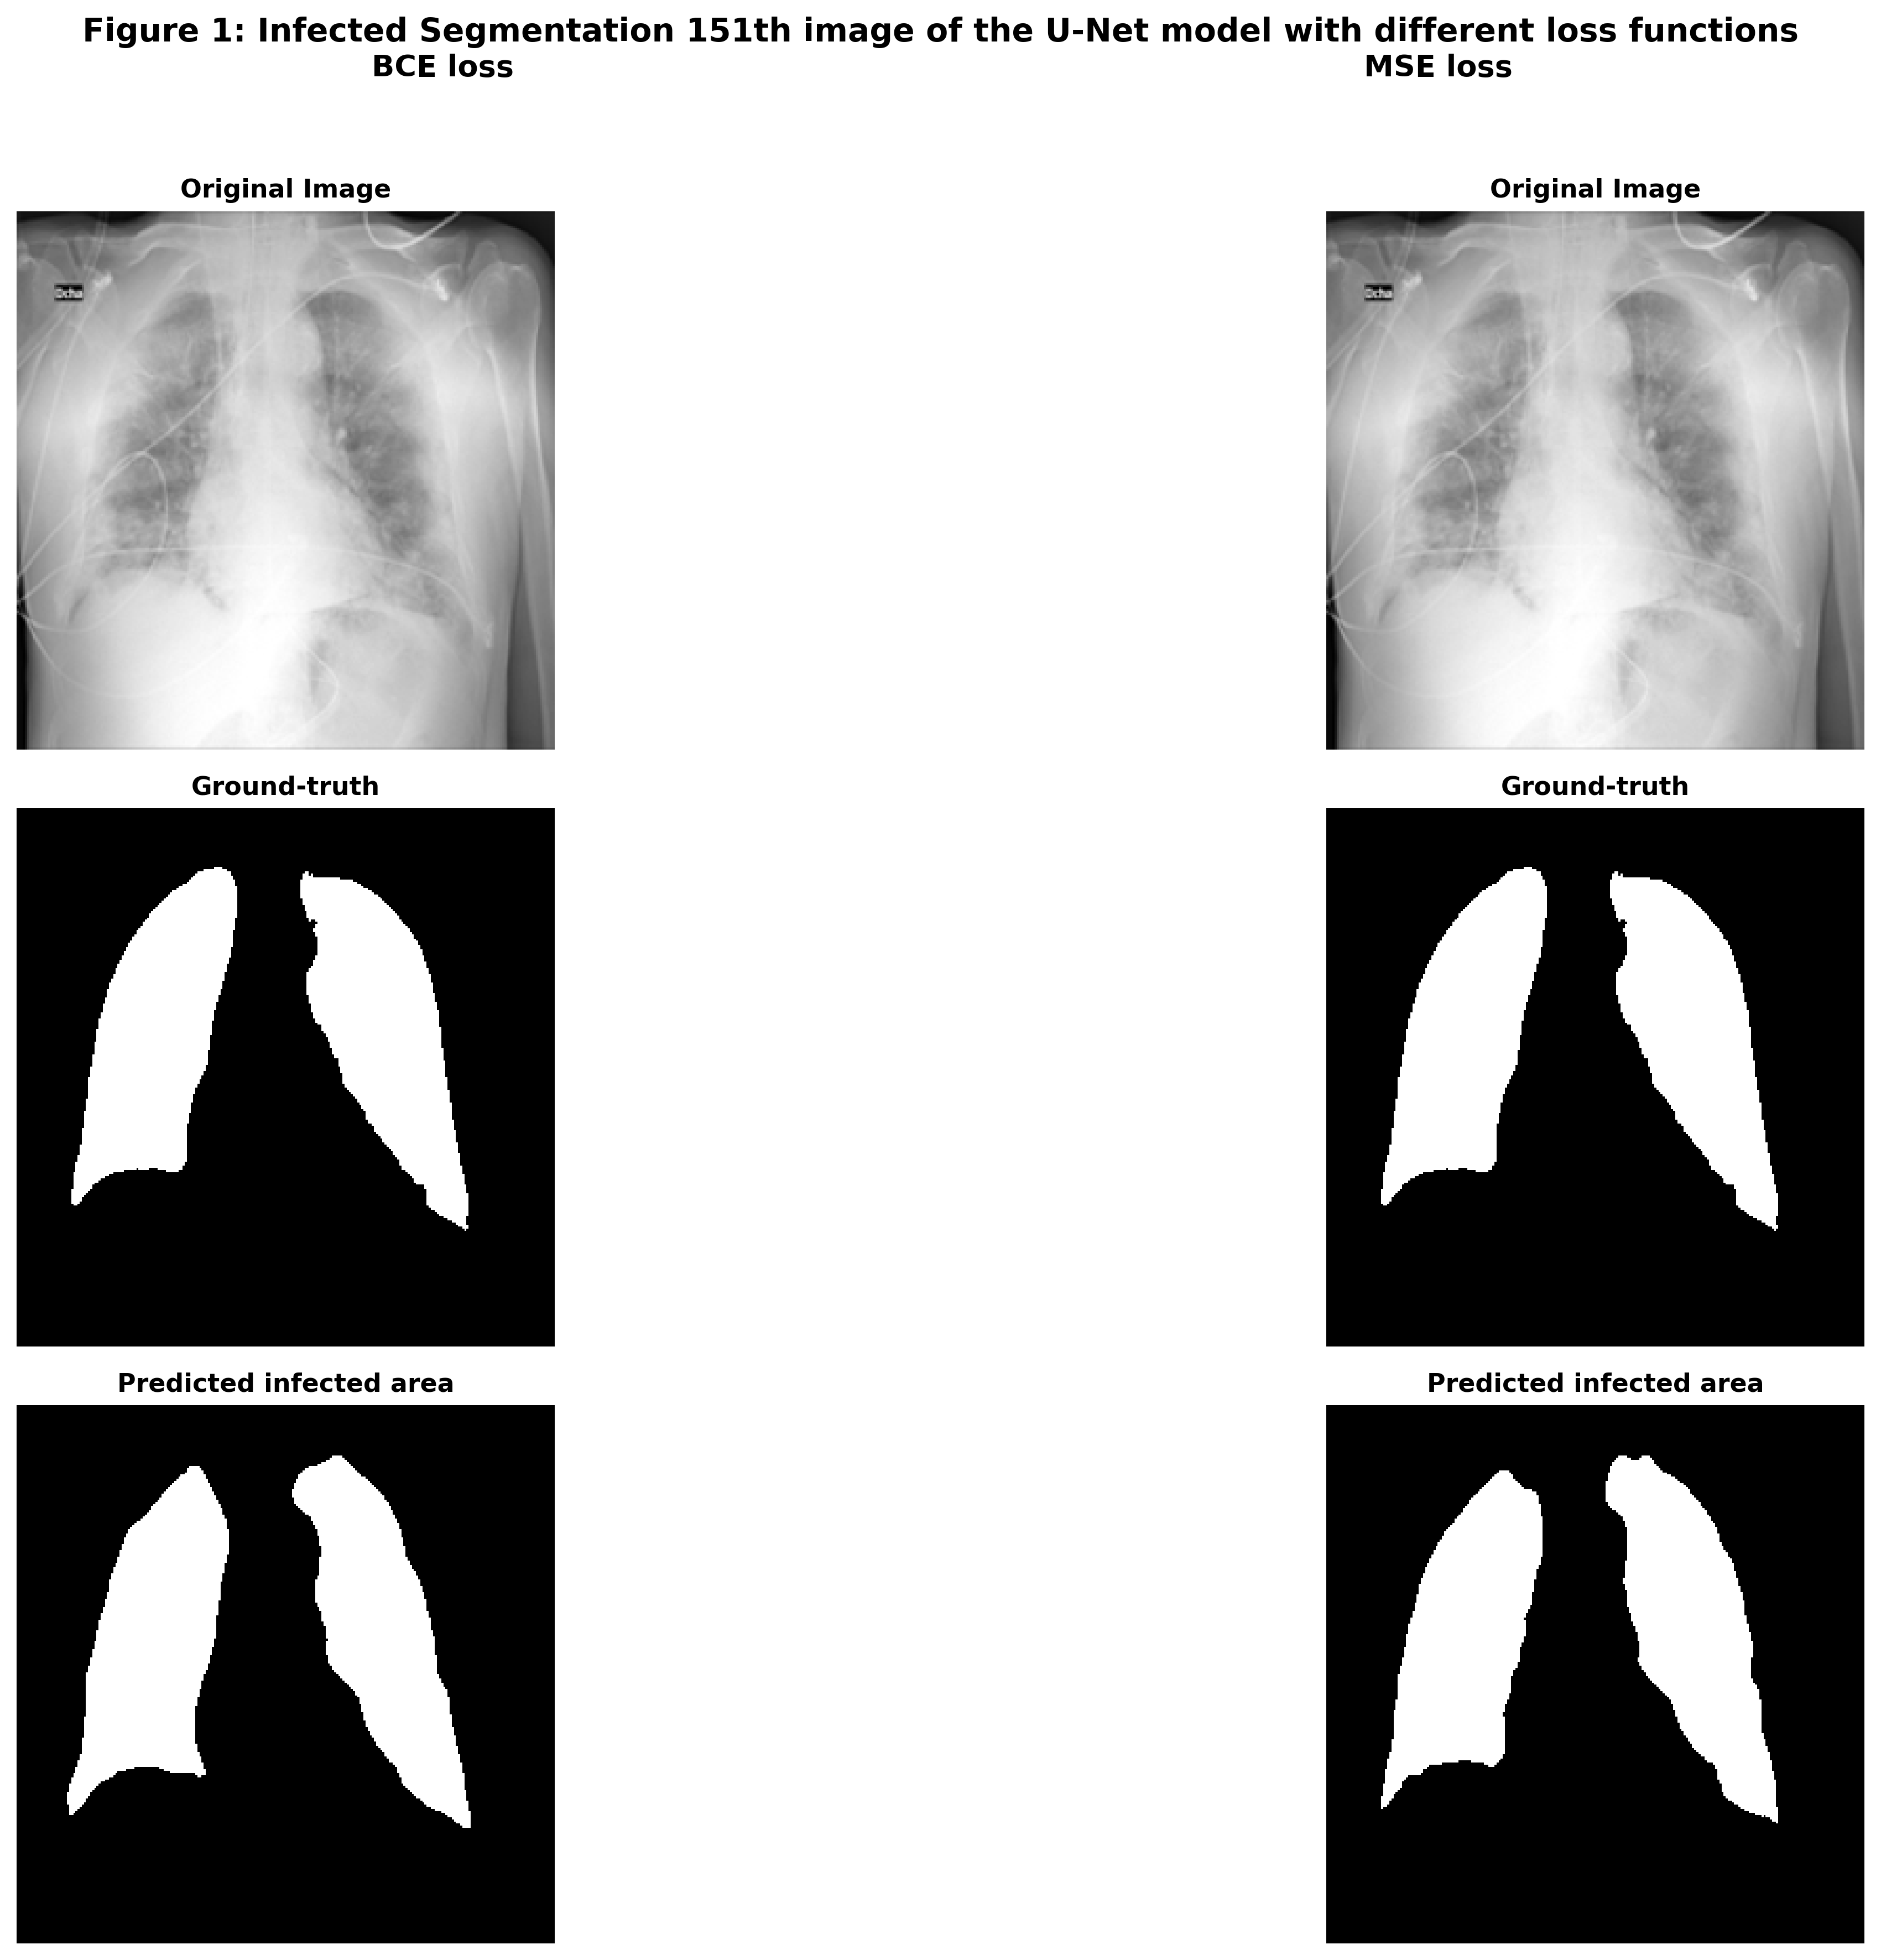
\includegraphics[width=0.9\columnwidth]{figure1_infected_segmentation_151th.png}
\caption{Example segmentation result in the 151th image}
\label{results}
\end{figure}

\begin{figure}[H]
\centering
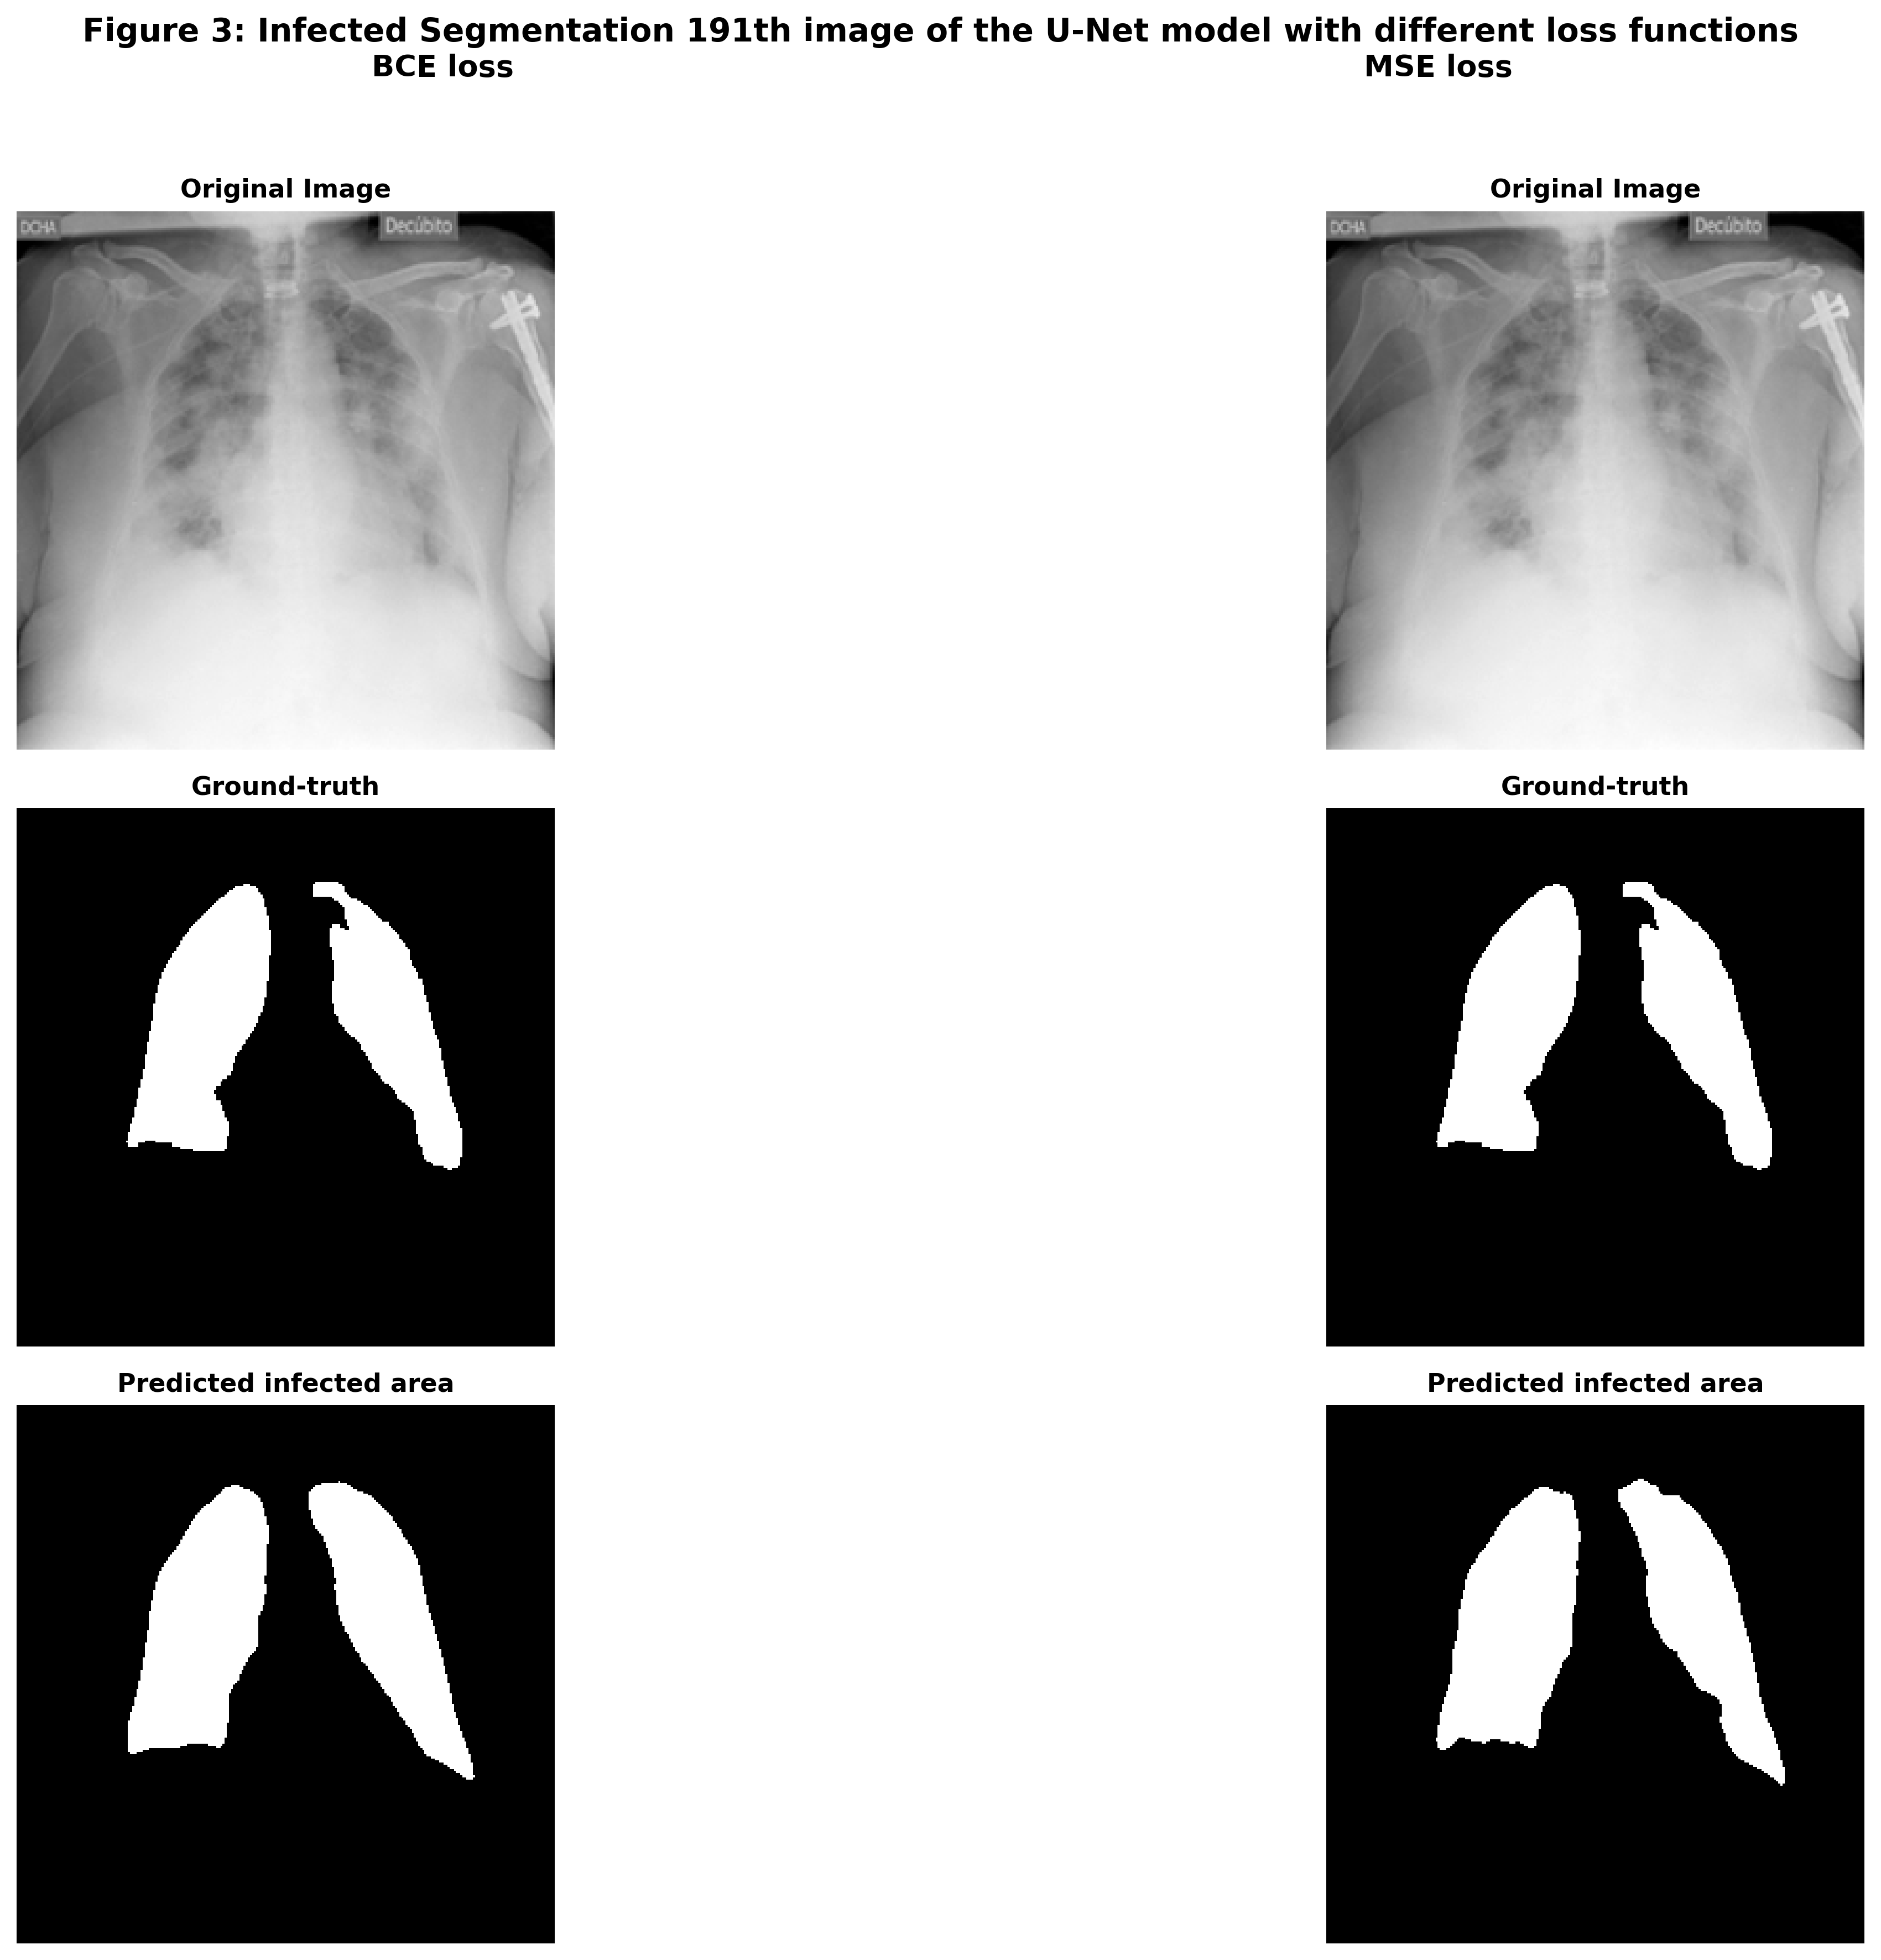
\includegraphics[width=0.8\columnwidth]{figure3_infected_segmentation_191th.png}
\caption{Example segmentation result in the 191th image}
\label{results}
\end{figure}

The model successfully identifies infection regions in most cases, although performance 
may degrade when infection areas are extremely small or have unclear boundaries.

Moreover, figure 3 shows the training and validation loss curves for the two loss functions used in this study, namely CrossEntropy and DiceCE. Both losses decrease over epochs, indicating that the model is able to learn meaningful representations.

For CrossEntropy, the training loss decreases steadily, while the validation loss shows noticeable fluctuations after several epochs, suggesting mild overfitting. In contrast, the DiceCE loss exhibits more stable behavior, with training and validation curves remaining closer throughout training. This indicates better generalization performance.

Overall, DiceCE provides more consistent convergence and is better suited for the segmentation task, as it accounts for both pixel-wise classification and region overlap.

\begin{figure}[H]
    \centering
    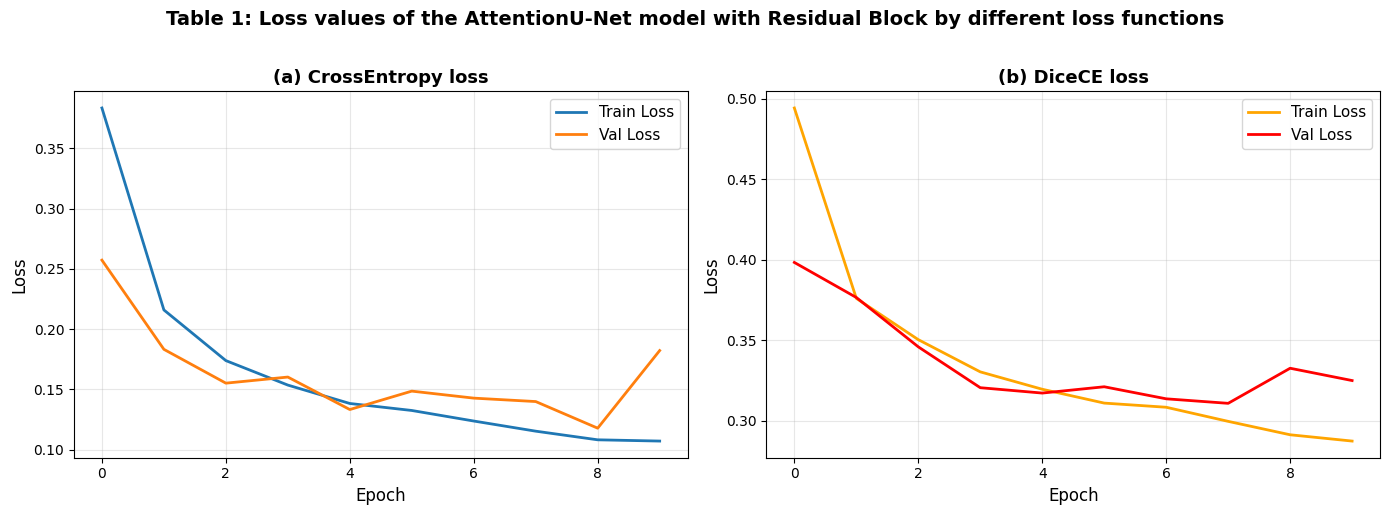
\includegraphics[width=\columnwidth]{medicineoutput.png}
    \caption{Training and validation loss curves using CrossEntropy and DiceCE.}
    \label{fig:loss_curves}
\end{figure}

\section{Comparison with State-of-the-Art}

We compare our model with existing segmentation methods reported in the literature.

\begin{table}[H]
\centering
\begin{tabular}{ccc}
\toprule
Method & Dice Score & IoU \\
\midrule
FPN + DenseNet 121 (Tahir et al., 2021) & 0.9611 & 0.9799 \\
ECA Attention-UNet with DANet & 0.9784 & 0.9740 \\
Proposed Model (CrossEntropy loss) & 0.8648 & 0.8122 \\
Proposed Model (DiceCE loss) & 0.8927 & 0.8404 \\
\bottomrule
\end{tabular}
\caption{Comparison with state-of-the-art models}
\end{table}

Our model achieves competitive performance while maintaining relatively low computational cost. Compared to more advanced architectures such as FPN combined with DenseNet121 and ECA Attention-UNet with DANet, the proposed model obtains slightly lower Dice and IoU scores. This difference can be attributed to the use of simpler architectural components and fewer parameters.

However, the proposed model still demonstrates strong segmentation capability, especially when using the DiceCE loss, which consistently outperforms the CrossEntropy loss in both Dice score and IoU. This confirms that incorporating overlap-based optimization improves performance for medical image segmentation tasks.

In addition, the simpler design of the proposed model makes it more efficient and easier to train, while still achieving reliable results. Therefore, it provides a good trade-off between performance and computational complexity, making it suitable for practical applications where resources may be limited.

\section{Conclusion}

This report presented a deep learning approach for COVID-19 infection segmentation using 
medical images.

The model demonstrates strong segmentation performance and highlights the effectiveness 
of convolutional neural networks for medical image analysis.

Future work could explore:

\begin{itemize}
\item Larger datasets
\item Transformer-based architectures
\item Improved loss functions
\end{itemize}

\end{document}
